\subsection{Comparing the permutations}
The performance of the six different functions resulting from the possibilities of permuting mnk are tested with square matrices with memory footprints ranging from a few kB to hundreds of MB. The results are seen in figure \ref{fig:comp1} with compiler option $\mathrm{-fast}$ enabled. The performance of the six functions behave in pairs depending on the last index which corresponds to the innermost for-loop. The functions pair up depending on this index because it is the loop being executed the most times, and so any performance issue coming from this loop is executed the most times as well. As seen in the figure \ref{fig:comp1}, the permutations with $m$ as the last index is a factor of $\sim 2$ slower than the other four permutations for memory footprints smaller than L2 cache. This is because $m$ is the column size of matrices $A$ and $C$, so by having the $m$ loop as the innermost loop, a lot of cache misses will happen due to C being a row major language, and looping along the columns as the fast loop will reduce the speed significantly. When the memory footprint exceeds the L2 cache size, the permutations with $k$ as the inner loop drops to the performance level of the permutations ending with $m$. The $k$-parameter is the row size of $A$ and column size of $B$, so in theory we should observe low performance, but it is likely that the compiler has optimized the structure in a way that is only beneficial as long as the data structures involved will fit on the L2 cache. Finally, the permutations with the $n$-loop as the fast loop perform well even when exceeding the L2 cache size. $n$ is the row size of $B$ and $C$, so looping over this variable fits well with C, and it gives the best possibilities for the compiler to optimize. When the L3 cache size is exceeded, the performance drops due to the fact that the data must now be transferred from the memory to the caches, and the bandwidth from the memory to the caches is much smaller than from cache to cache. The drop is not large, so it is possible that the compiler utilizes prefetching to reduce the effect of the decreased bandwidth. It is also worth noting that mkn performs better than kmn for all memory footprints, and the reason here is that the loop over $m$ is the slowest, and thus to achieve the best performance, this loop must placed as the outmost loop.

\subsubsection{Analyzer tool}
We expect better-performing permutations to have less cache misses.   To validate our hypotheses regarding cache hits we conducted a profiling experiment. That is, we fixed the matrix dimension size to 724 which corresponds to ~12MB memory footprint, ran each of the six permutations (without compiler optimizations) using the collect command and viewed the results using Oracle Solaris Studio Performance Analyzer. To be able to make direct comparisons, we set the minimum runtime to zero and max iterations to one. This way each permutation is run for a single iteration and we can compare cache hits in absolute terms. \\
Level 1 and 2 cache hits and misses as well as CPU time of the permutations are presented in table \ref{tab:tab1}.
\begin{center}
\captionof{table}{Cache counters in millions with 12MB memory footprint} \label{tab:tab1} 
\begin{tabular}{ |c|c|c|c|c|c| } 
\hline
 & L1d hit & L1d miss & L2 hit & L2 miss & CPU time \\ 
\hline
nkm & 6849 & 755 & 704 & 50 & 2.410 \\  
\hline
nmk & 7229 & 373 & 373 & 1 & 2.030 \\ 
\hline
mkn & 7599 & 0 & 0 & 0 & 1.810 \\ 
\hline
mnk & 7229 & 376 & 328 & 47 & 2.310 \\ 
\hline
knm & 6849 & 755 & 704 & 51 & 2.350 \\ 
\hline
kmn & 7599 & 0 & 0 & 0 & 1.820 \\ 
\hline
\end{tabular}
\end{center}

Interpret results of table


When the memory footprint 

\begin{figure}
\centering
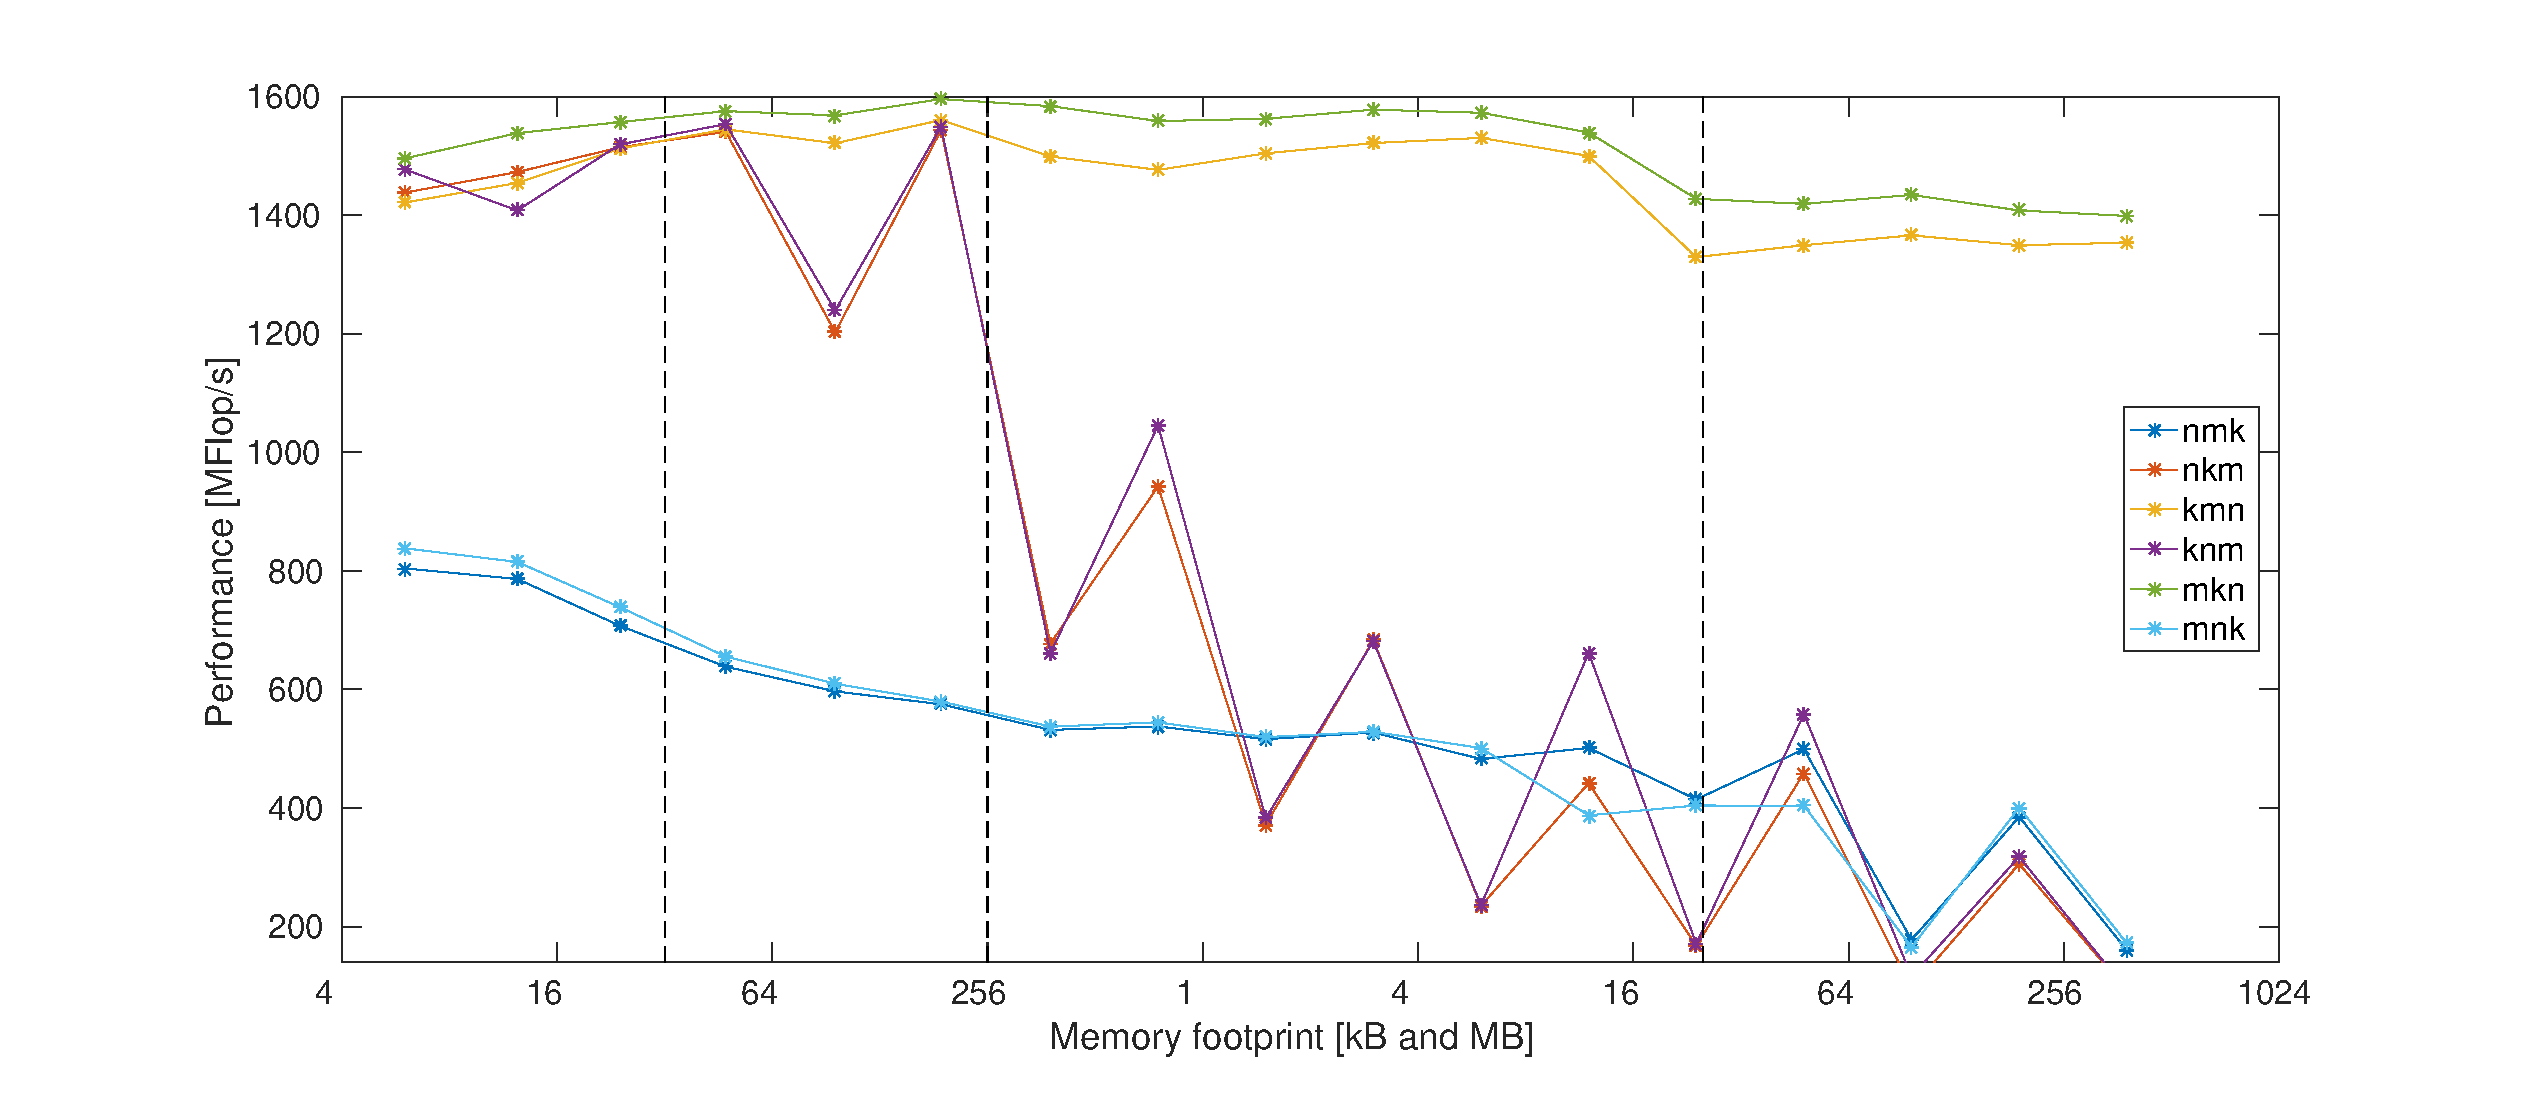
\includegraphics[width = 1.1\textwidth]{fig/permGraph_fast.eps}
\caption{This is a caption}
\label{fig:comp1}
\end{figure}

\begin{itemize}
\item hpcintro queue node cpu information
\item Introduce functions
\item Show library vs. native
\item introduce the permutations WITHOUT -fast and show the performance vs. memory footprint for all permutations
\item Optimize by compiler options (-fast, -O3, -prefetch etc. etc.)
\item Performace Analyzer tool experiment(s), relate results to  memory footprint-performance plot.
\item Blocking and find optimum block size
\item Compare blocking to the best w/o blocking
\end{itemize}
